\documentclass[12pt, titlepage]{article}

\usepackage{booktabs}
\usepackage{tabularx}
\usepackage{hyperref}
\hypersetup{
    colorlinks,
    citecolor=black,
    filecolor=black,
    linkcolor=red,
    urlcolor=blue
}
\usepackage[round]{natbib}
\usepackage{fullpage}
\usepackage{scrextend}
\usepackage{amsmath}
\usepackage{graphicx}
\usepackage[dvipsnames]{xcolor}
\graphicspath{ {image/} }


\newcommand{\progname}{SpecGen}

\newcounter{testnum} %Instance Number
\newcommand{\tthetestnum}{T\thetestnum}
\newcommand{\testref}[1]{T\ref{#1}}
\newcommand{\sref}[1]{\S~\ref{#1}}


\begin{document}
\pagenumbering{gobble}

\title{CAS 741: Test Report\\[10pt]\Large Aqueous Speciation Diagram Generator}
\author{Steven Palmer\\\texttt{palmes4}}
\date{\today}
	
\maketitle

\pagenumbering{roman}

\setcounter{secnumdepth}{0}

\section{Revision History}

\begin{table}[hp]
\caption{Revision History} \label{TblRevisionHistory}
\begin{tabularx}{\textwidth}{llX}
\toprule
\textbf{Date} & \textbf{Developer(s)} & \textbf{Change}\\
\midrule
12.18.2017 & S. Palmer & Revision 1\\
\bottomrule
\end{tabularx}
\end{table}

\newpage

\tableofcontents


\newpage


\pagenumbering{arabic}

\setcounter{secnumdepth}{3}

This document gives the results of the testing proposed in the
\progname{} Test Plan document (found 
\href{https://github.com/palmerst/cas741_sp/blob/master/Doc/TestPlan/TestPlan.pdf}{here}).


\section{Functional Requirements Evaluation}

\subsection{Automated Tests}
\noindent {\bf T\refstepcounter{testnum}\thetestnum \label{T_DiagFe}: 
Diagram generation of FeOH$_3$ system:}~
{\color{Green} \bf PASS}\\
\noindent {\bf T\refstepcounter{testnum}\thetestnum \label{T_DiagCO2}: 
Diagram generation of CO$_2$ system:}~
{\color{Green} \bf PASS}

\subsection{Manual Tests}
\noindent {\bf T\refstepcounter{testnum}\thetestnum \label{T_Comp}: 
Comparison of 
generated speciation diagram to original:}~
{\color{Green} \bf PASS}\\[\baselineskip]
{\bf Remarks:} The output of the original MATLAB implementation is shown
in \hyperref[fig:orig]{Figure~\ref*{fig:orig}} and the output of \progname{}
is shown in \hyperref[fig:gen]{Figure~\ref*{fig:gen}} (see Appendix).  A visual
inspection of these diagrams reveals that they are the same.  Note that the y-axis
is different between these diagrams.  This is not a problem since ``fraction of
total Fe'' is simply the concentration divided by the total amount of Fe in the system.
The total amount of Fe is a constant, and thus the shape of the curves is not affected.

\section{Nonfunctional Requirements Evaluation}
\subsection{Manual Tests}
\noindent {\bf T\refstepcounter{testnum}\thetestnum \label{T_NF_Read}: Readability of 
generated speciation diagram:}~{\color{Green} \bf PASS}\\[\baselineskip]
{\bf Remarks:}  The \progname{} output for the FeOH$_3$ system is given in 
\hyperref[fig:gen]{Figure~\ref*{fig:gen}} (see Appendix).  Upon visual inspection,
the title, axis labels, legend, and curves are all easily read, as required.


\section{Unit Testing}
\noindent {\bf T\refstepcounter{testnum}\thetestnum 
\label{T_Plot}: Plotting test:}~{\color{Green} \bf PASS}\\
\noindent {\bf T\refstepcounter{testnum}\thetestnum 
\label{T_ConvFe}: Input conversion of FeOH$_3$ system:}~{\color{Green} \bf PASS}\\
\noindent {\bf T\refstepcounter{testnum}\thetestnum 
\label{T_ConvCO2}: Input conversion of CO$_2$ system:}~{\color{Green} \bf PASS}\\
\noindent {\bf T\refstepcounter{testnum}\thetestnum 
\label{T_ConvExc}: Input conversion of empty system:}~{\color{Green} \bf PASS}\\
\noindent {\bf T\refstepcounter{testnum}\thetestnum 
\label{T_CalcExc}: Calculation of empty system:}~{\color{Green} \bf PASS}\\
\noindent {\bf T\refstepcounter{testnum}\thetestnum 
\label{T_CalcLine}: Calculation of simple system:}~{\color{Green} \bf PASS}\\
\noindent {\bf T\refstepcounter{testnum}\thetestnum 
\label{T_SysBad1}: Register reaction as empty string:}~{\color{Green} \bf PASS}\\
\noindent {\bf T\refstepcounter{testnum}\thetestnum 
\label{T_SysBad2}: Register reaction without equilibrium constant:}~{\color{Green} \bf PASS}\\
\noindent {\bf T\refstepcounter{testnum}\thetestnum 
\label{T_SysBad3}: Register reaction without products:}~{\color{Green} \bf PASS}\\
\noindent {\bf T\refstepcounter{testnum}\thetestnum 
\label{T_SysBad4}: Register reaction with bad state:}~{\color{Green} \bf PASS}\\
\noindent {\bf T\refstepcounter{testnum}\thetestnum 
\label{T_SysBad5}: Register reaction with bad formula (non-letter symbol):}~{\color{Green} \bf PASS}\\
\noindent {\bf T\refstepcounter{testnum}\thetestnum 
\label{T_SysBad6}: Register reaction with bad formula (beginning with lower case):}~{\color{Green} \bf PASS}\\
\noindent {\bf T\refstepcounter{testnum}\thetestnum 
\label{T_SysBad7}: Register reaction with bad formula (no parentheses):}~{\color{Green} \bf PASS}\\
\noindent {\bf T\refstepcounter{testnum}\thetestnum 
\label{T_SysBad8}: Register reaction with bad formula (unbalanced parentheses):}~{\color{Green} \bf PASS}\\
\noindent {\bf T\refstepcounter{testnum}\thetestnum 
\label{T_SysParen1}: Register reaction with superfluous parentheses:}~{\color{Green} \bf PASS}\\
\noindent {\bf T\refstepcounter{testnum}\thetestnum 
\label{T_SysParen2}: Register reaction with high parenthesis nesting:}~{\color{Green} \bf PASS}\\
\noindent {\bf T\refstepcounter{testnum}\thetestnum 
\label{T_TotNeg}: Register negative element total:}~{\color{Green} \bf PASS}\\
\noindent {\bf T\refstepcounter{testnum}\thetestnum 
\label{T_TotZero}: Register zero element total:}~{\color{Green} \bf PASS}\\
\noindent {\bf T\refstepcounter{testnum}\thetestnum 
\label{T_TotPos}: Register positive element total:}~{\color{Green} \bf PASS}

\section{Changes Due to Testing}
Testing was carried out throughout development, with changes made
to ensure \progname{} behaved as expected.

\section{Automated Testing}
The output of the automated test suite is shown in \hyperref[fig:results]{Figure~\ref*{fig:results}}.
All automated tests passed.

\begin{figure}[!h]
\centering
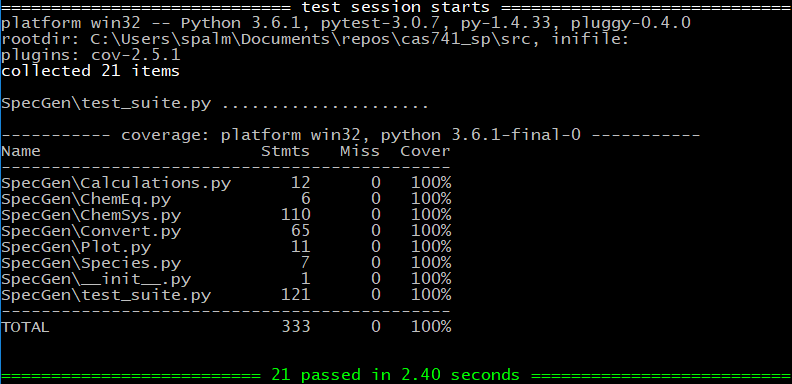
\includegraphics[width=\textwidth]{results}
\caption{Automated testing results} \label{fig:results}
\end{figure}
		
\section{Trace to Requirements}
A trace between system tests and requirements is provided in 
\hyperref[tab:reqtrace]{Table~\ref*{tab:reqtrace}}.

\begin{table}[h]
\caption{Requirements Traceability} \label{tab:reqtrace}
\centering
\begin{tabularx}{0.55\textwidth}{p{4cm}X}
\toprule {\bf Requirement} & {\bf Test(s)}\\
\midrule
R1	&	\testref{T_DiagFe}, \testref{T_DiagCO2}, \testref{T_Comp}\\
R2	&	\testref{T_DiagFe}, \testref{T_DiagCO2}, \testref{T_Comp}\\
R3	&	\testref{T_DiagFe}, \testref{T_DiagCO2}, \testref{T_Comp}\\
R4	&	\testref{T_DiagFe}, \testref{T_DiagCO2}, \testref{T_Comp}\\
R5	&	\testref{T_DiagFe}, \testref{T_DiagCO2}, \testref{T_Comp}\\
NF1 & \testref{T_NF_Read}\\
\bottomrule
\end{tabularx}
\end{table}		
		
\section{Trace to Modules}		
A trace between unit tests and modules is provided in 
\hyperref[tab:modtrace]{Table~\ref*{tab:modtrace}}.

\begin{table}[h]
\caption{Module Traceability} \label{tab:modtrace}
\centering
\begin{tabularx}{0.90\textwidth}{lX}
\toprule {\bf Module} & {\bf Test(s)}\\
\midrule
M1 & implemented by OS; no tests required\\
M2 & external interface; no explicit testing; covered implicitly\\
M3 & \testref{T_SysBad1}, \testref{T_SysBad2}, \testref{T_SysBad3}, 
\testref{T_SysBad4}, \testref{T_SysBad5}, \testref{T_SysBad6}, 
\testref{T_SysBad7}, \testref{T_SysBad8}, \testref{T_SysParen1},
\testref{T_SysParen2}, \testref{T_TotNeg}, \testref{T_TotZero},
\testref{T_TotPos} \\
M4 & data structure; no explicit testing; covered implicitly\\
M5 & data structure; no explicit testing; covered implicitly\\
M6 & \testref{T_ConvFe}, \testref{T_ConvCO2}, \testref{T_ConvExc}\\
M7 & \testref{T_CalcExc}, \testref{T_CalcLine}\\
M8 & implemented by Python; no tests required\\
M9 & \testref{T_Plot}\\
\bottomrule
\end{tabularx}
\end{table}

\section{Code Coverage Metrics}
The results of the code coverage analysis is shown in Figure~\ref{fig:results}.
The target of 100\% code coverage for the automated testing was successfully met. 

\newpage
\section{Appendix}
\begin{figure}[!h]
\centering
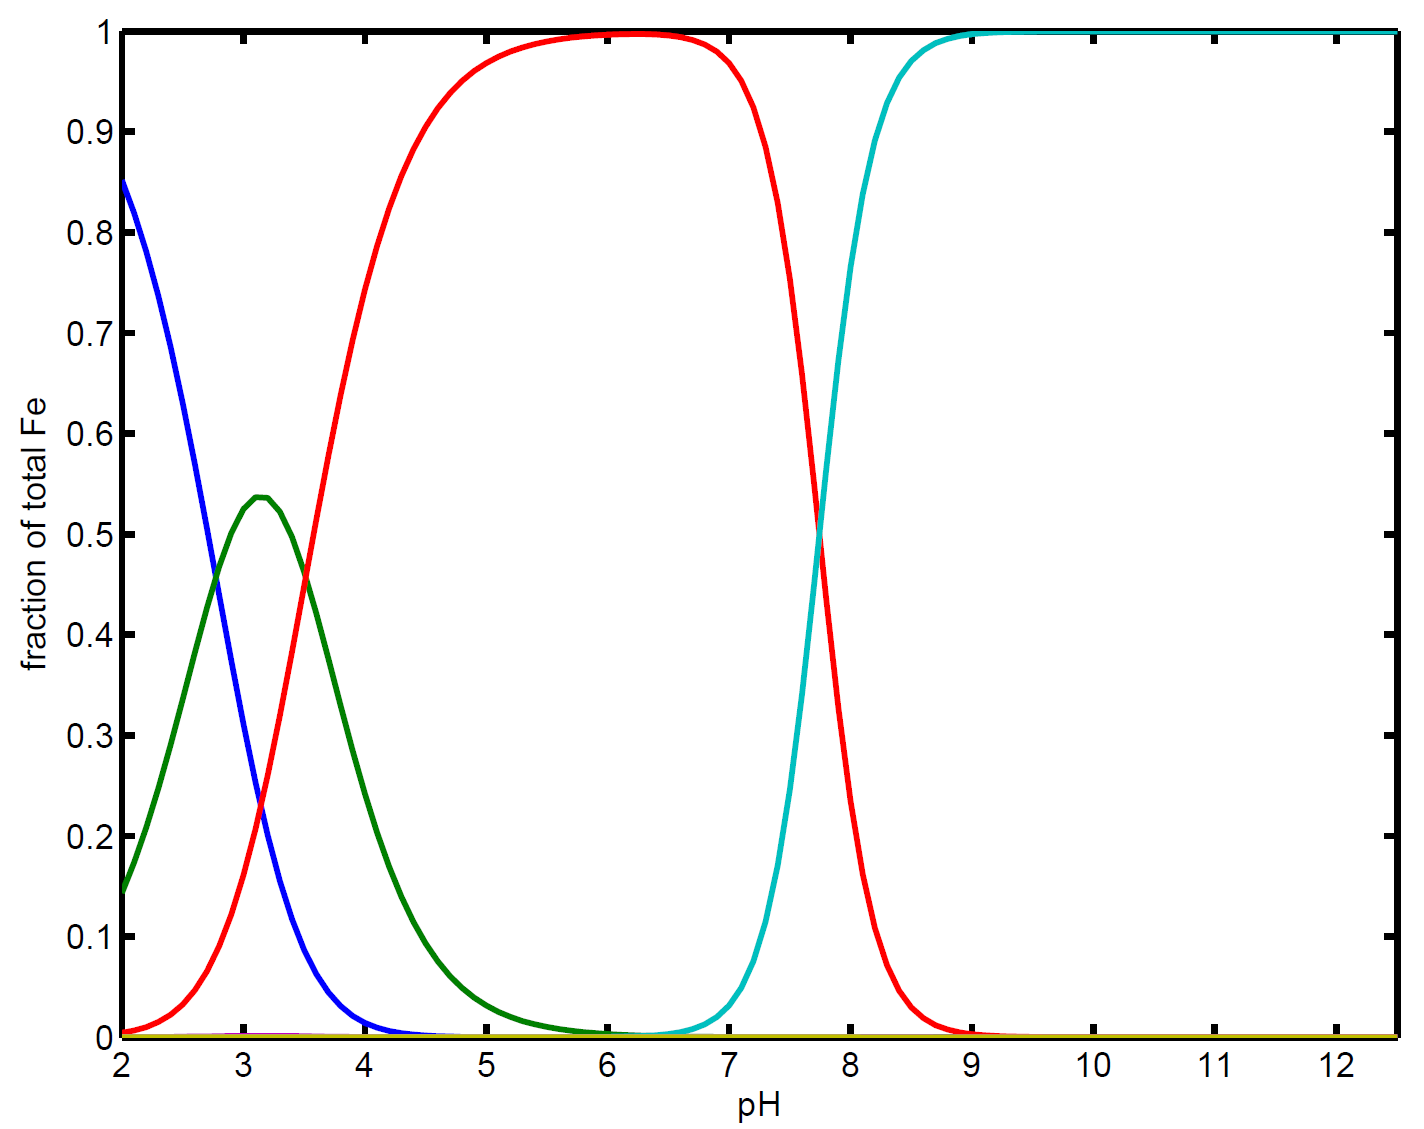
\includegraphics[width=\textwidth]{orig_ref}
\caption{Dr. Smith's MATLAB implementation output for FeOH$_3$ system} \label{fig:orig}
\end{figure}
\begin{figure}[!h]
\centering
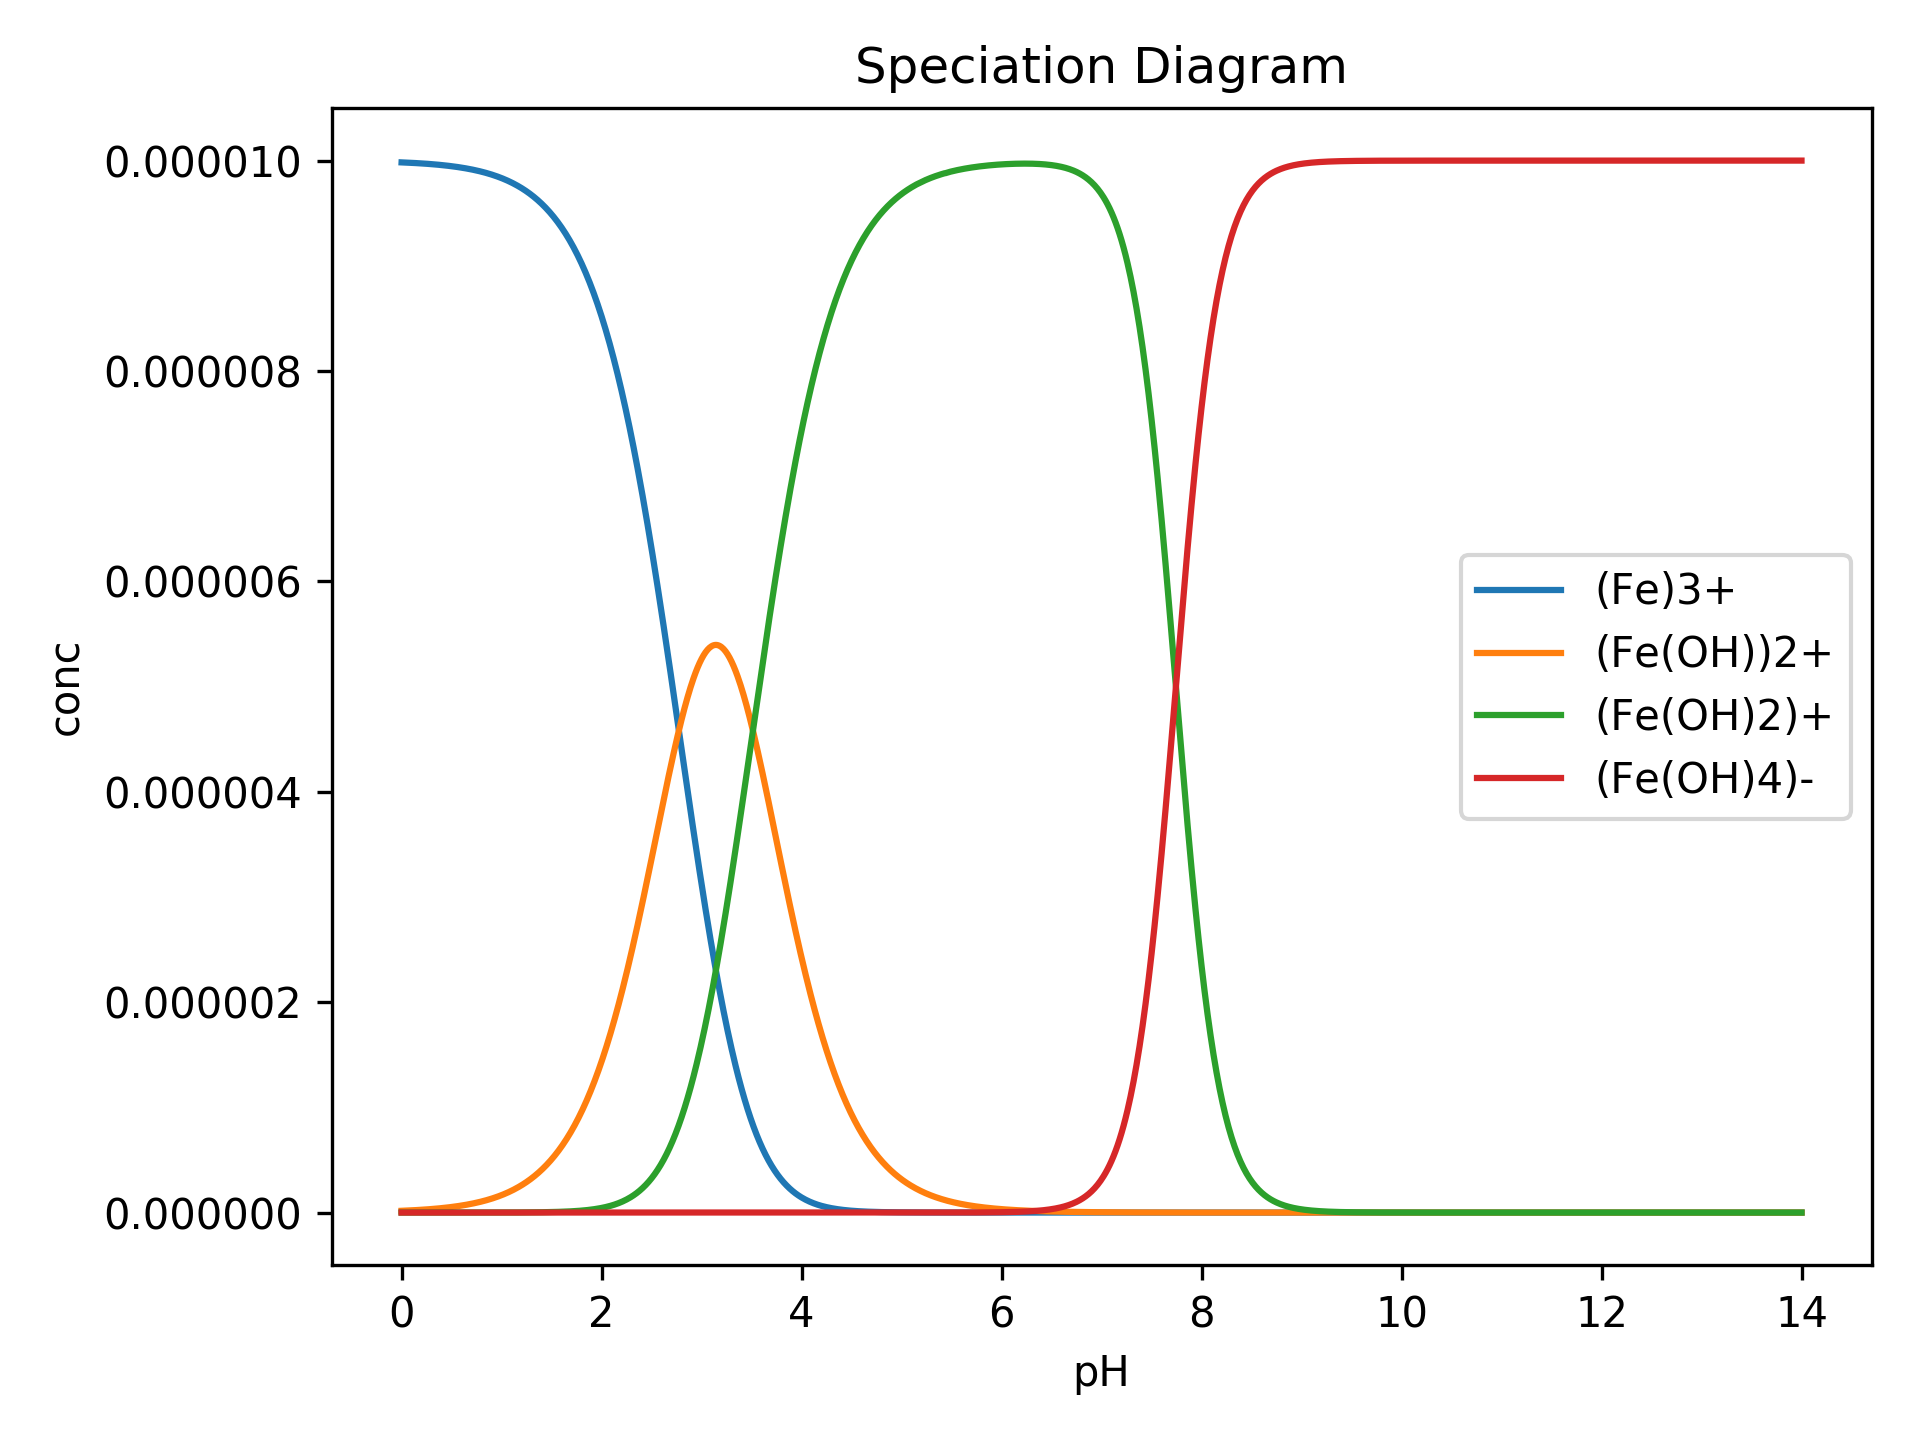
\includegraphics[width=\textwidth]{fe_syst}
\caption{\progname{} output for FeOH$_3$ system} \label{fig:gen}
\end{figure}
\end{document}
